\chapter{Componentes}

% http://itp.nyu.edu/physcomp/Labs/Components
\section{Voltage Regulator}

Voltage regulators take a range of DC voltage and convert it to a constant voltage. For example, this regulator, a 7805 regulator, takes a range of 8 - 15 volts DC input and converts it to a constant 5-volt output.

Note the label on the regulator that reads "7805". Check the label on every component. This physical form factor, called the package, is used by many different components, and not all of them are voltage regulators. This is a TO-220 package.

The 7800 series regulators come in many different voltages. 7805 is a 5-volt regulator. 7809 is a 9-volt regulator. 7812 is a 12-volt regulator. All the regulators of this family have the same pin connections. In the image above, the left leg is connected to the input voltage. The middle leg is connected to ground. The right leg is the output voltage.

\href{http://www.national.com/ds.cgi/LM/LM341.pdf}{7805 datasheet}

\begin{figure}[!htb]
     \centering
     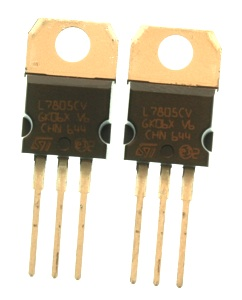
\includegraphics[scale=0.3]{img/components/v_reg_7805.jpg}
     \caption{5V voltage regulator}
     \label{5V voltage regulator}
\end{figure}

\begin{figure}[!htb]
     \centering
     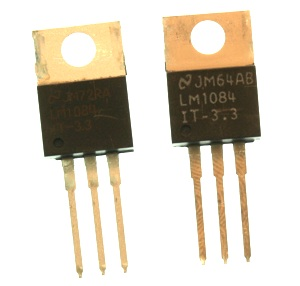
\includegraphics[scale=0.3]{img/components/v_reg_33v.jpg}
     \caption{3.3V voltage regulator}
     \label{3.3V voltage regulator}
\end{figure}

3.3V regulators are also common. Note that these ones don't have the same pin configuration as the 7805 regulators!

\section{LED}

\begin{figure}[!htb]
     \centering
     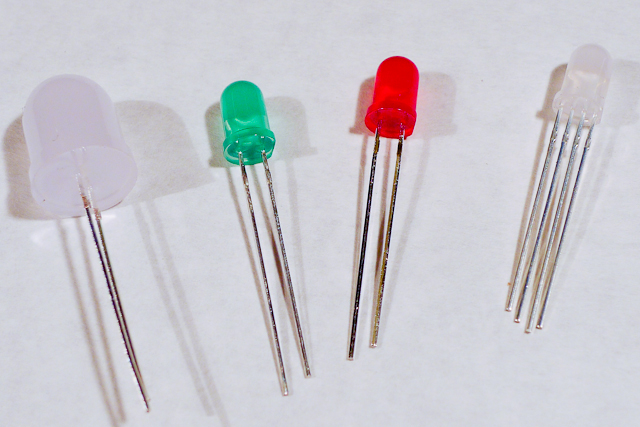
\includegraphics[scale=0.3]{img/components/leds.jpg}
     \caption{LEDs}
     \label{LEDs}
\end{figure}

LEDs, or Light Emitting Diodes, are diodes that emit light when given the correct voltage. Like all diodes, they are polarized, meaning that they only operate when oriented correctly in the circuit. The anode of the LED connects to voltage, and the cathode connects to ground. The anode in the LEDs in this photo is the longer leg on each LED. LEDs come in many diferent packages. The packages above have built-in lenses.
These LEDs are the cheapest you can buy, and they're not very bright. You can get superbright LEDs as well, which are much brighter. If you're working on applications that need very small light sources, you can also get LEDs in a surface mount package.
LEDs can only handle a limited amount of current and voltage. The details should be covered in each LED's datasheet, but if not, here's a link to a handy LED current calculator. For most common LEDs running at 5 volts, a resistor between 220 and 1K ohms will do the job.

\begin{figure}[!htb]
     \centering
     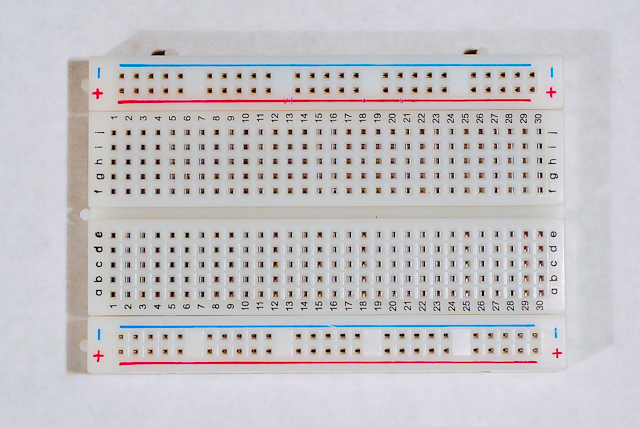
\includegraphics[scale=0.55]{img/components/breadboard_short.jpg}
     \caption{solderless breadboard}
     \label{solderless breadboard}
\end{figure}



\section{Resistors}

Resistors resist the flow of electrical current. When placed in series, they reduce the voltage, and limit the current. The bands on a resistor indicate the resistor's value. Here's a handy resistor color code calculator. 

\begin{figure}[!htb]
     \centering
     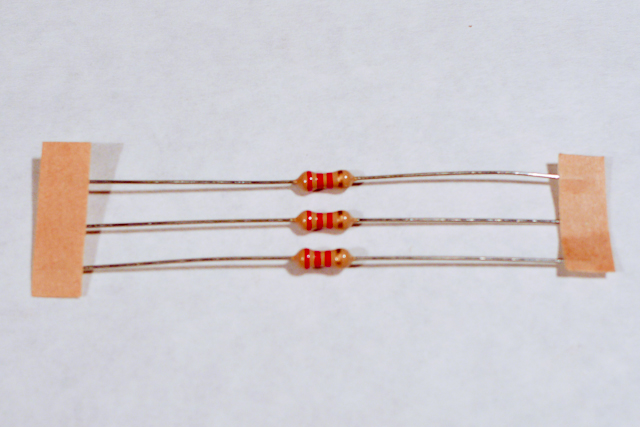
\includegraphics[scale=0.3]{img/components/resistors.jpg}
     \caption{resistors}
     \label{resistors}
\end{figure}

\section{Potentiometers}


Potentiometers are variable resistors. The two outside terminals act as a fixed resistor. A movable contact called the wiper moves across the resistor, producing a variable resistance between the center terminal and either of the two sides. 

\begin{figure}[!htb]
     \centering
     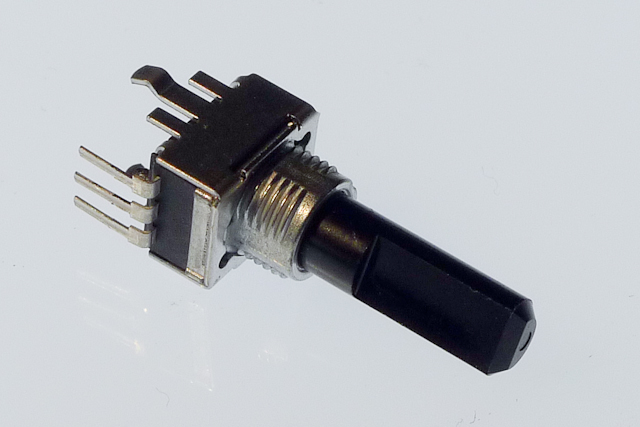
\includegraphics[scale=0.25]{img/components/potentiometer.jpg}
     \caption{potentiometer}
     \label{potentiometer}
\end{figure}

\subsection{trimmer potentiometers}
Trimmer potentiometers are designed to be mounted on a circuit board, difficult to turn, so you can use them to adjust a circuit. They're handy to use as physical variables, to tune your project. 

\begin{figure}[!htb]
     \centering
     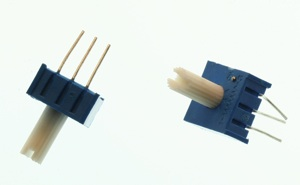
\includegraphics[scale=0.3]{img/components/pots_trimmer.jpg}
     \caption{trimmer potentiometer}
     \label{trimmer potentiometer}
\end{figure}

\section{Switches}

Switches are one form of digital input. There are many kinds of switches. The two most useful caategories are \textbf{momentary switches}, which remain closed only when you press them, and \textbf{toggle switches}, which stay in place after you switch them. 

\begin{figure}[!htb]
     \centering
     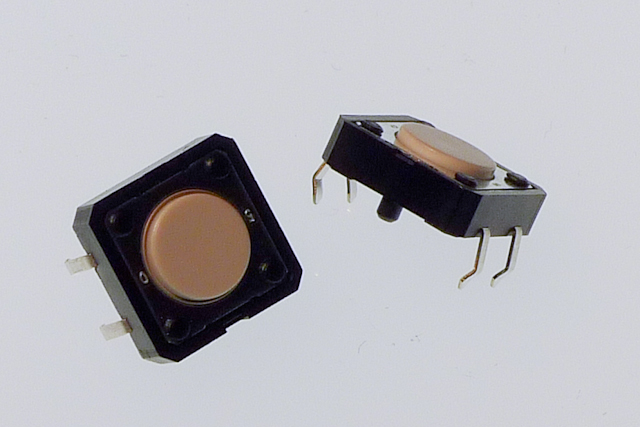
\includegraphics[scale=0.3]{img/components/switches_momentary.jpg}
     \caption{momentary switches}
     \label{momentary switches}
\end{figure}

\begin{figure}[!htb]
     \centering
     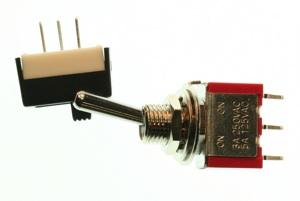
\includegraphics[scale=0.3]{img/components/switches_toggle.jpg}
     \caption{toggle switches}
     \label{toggle switches}
\end{figure}

\section{Photocells}

Photocells are variable resistors whose resistance changes as the light hitting them changes.

\begin{figure}[!htb]
     \centering
     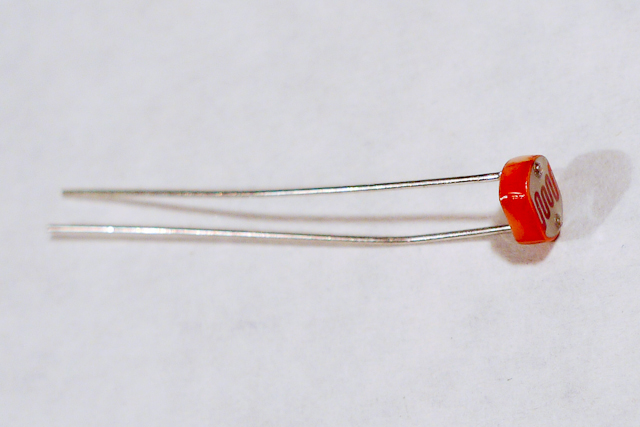
\includegraphics[scale=0.3]{img/components/photocell.jpg}
     \caption{photocell}
     \label{photocell}
\end{figure}

\section{Thermistors}

Thermistors are variable resistors whose resistance changes as the temperature changes. 

\begin{figure}[!htb]
     \centering
     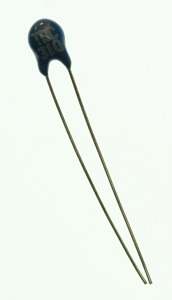
\includegraphics[scale=0.5]{img/components/thermistor.jpg}
     \caption{thermistor}
     \label{thermistor}
\end{figure}



\section{Capacitors}

Capacitors store electrical energy while there's energy coming in, and release it when the incoming energy stops. They have a variety of uses. One common use is to smooth out the dips and spikes in an electrical supply. This use is called decoupling.

\begin{figure}[!htb]
     \centering
     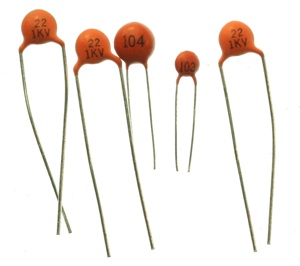
\includegraphics[scale=0.3]{img/components/caps_ceramic.jpg}
     \caption{ceramic capacitors}
     \label{ceramic capacitors}
\end{figure}

LEDs, or Light Emitting Diodes, are diodes that emit light when given the correct voltage. Like all diodes, they are polarized, meaning that they only operate when oriented correctly in the circuit. The anode of the LED connects to voltage, and the cathode connects to ground. The anode in the LEDs in this photo is the longer leg on each LED. LEDs come in many diferent packages. The packages above have built-in lenses.

\begin{figure}[!htb]
     \centering
     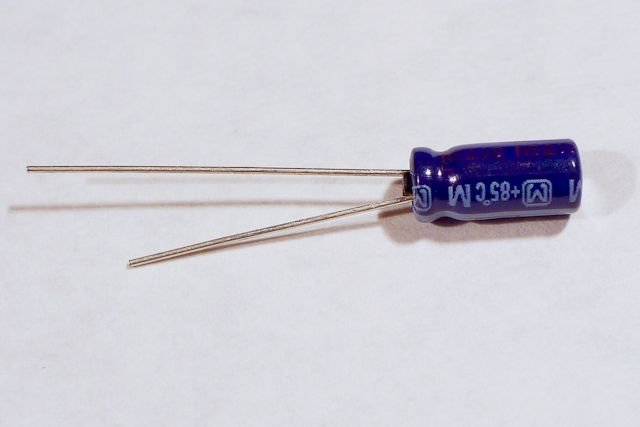
\includegraphics[scale=0.3]{img/components/caps_electrolytic.jpg}
     \caption{electrolytic capacitors}
     \label{electrolytic capacitors}
\end{figure}

Ceramic capacitors are cheap and unpolarized. They generally have very small capaacitance values. They're useful decoupling caps in a low-current circuit. You often see them used to decouple the power going into a microcontroller or other integrated circuit.
The number on a ceramic cap gives you its value and order of magnitude. For example, 104 indicates a 0.1 microfarad (uF) cap. 103 indicates a 0.001 microfarad cap. 

\begin{figure}[!htb]
     \centering
     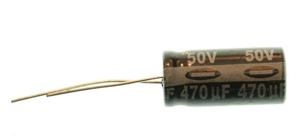
\includegraphics[scale=0.3]{img/components/cap_electrolytic_detail.jpg}
     \caption{electrolytic capacitor detail}
     \label{electrolytic capacitor detail}
\end{figure}


Electrolytic capacitors can generally store more charge than ceramic caps, and are longer lasting and more expensive. They're usually polarized, meaning that they have a positive leg and a negative leg. This is because current flows more efficiently through them one way than the other. 

An electrolytic cap will have a + or - on one side, as shown here. 

\section{Diodes}

\begin{figure}[!htb]
     \centering
     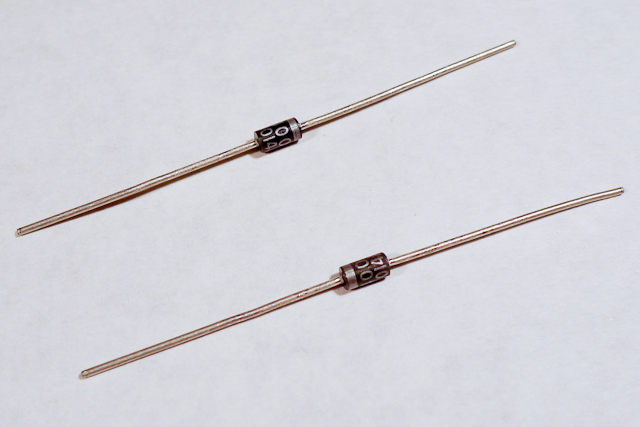
\includegraphics[scale=0.3]{img/components/diodes_400x.jpg}
     \caption{1N4001 diodes}
     \label{1N4001 diodes}
\end{figure}

Diodes permit voltage to flow in one direction and block it in the other direction. LEDs are a type of diode, as are the 1N4001 diodes shown here. They're useful for stopping voltage from going somewhere you don't want it to go. 

\begin{figure}[!htb]
     \centering
     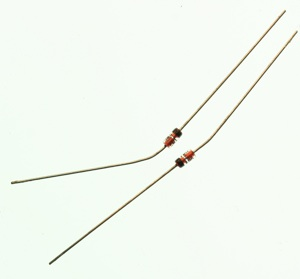
\includegraphics[scale=0.3]{img/components/diodes_zener.jpg}
     \caption{zener diodes}
     \label{zener diodes}
\end{figure}


Zener diodes have a breakdown voltage past which they allow current to flow in both directions. They're used to chop off excess voltage from a part of a circuit.

\section{Transistors}

\begin{figure}[!htb]
     \centering
     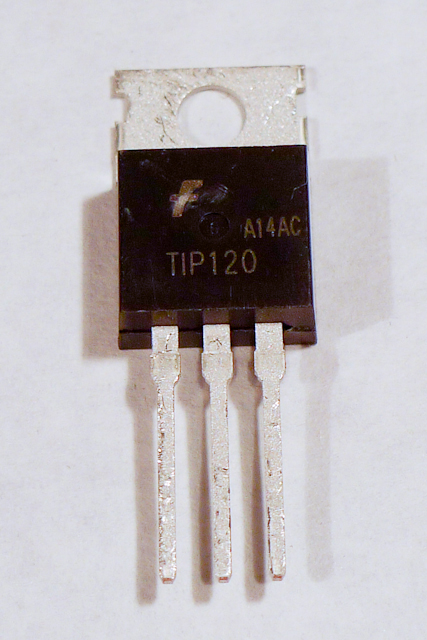
\includegraphics[scale=0.3]{img/components/transistors.jpg}
     \caption{transistors}
     \label{transistors}
\end{figure}

Transistors act as electronic switches. When you put a small voltage across the base and emitter, the transistor allows a larger current and voltage to flow from the collector to the emitter.

\section{Power Jacks}

\begin{figure}[!htb]
     \centering
     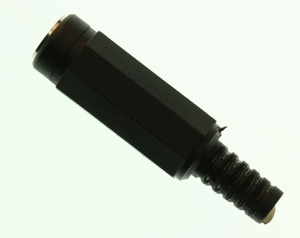
\includegraphics[scale=0.5]{img/components/power_jack.jpg}
     \caption{DC power jack, disassembled}
     \label{DC power jack, disassembled}
\end{figure}

\begin{figure}[!htb]
     \centering
     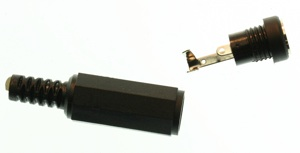
\includegraphics[scale=0.3]{img/components/power_jack_2.jpg}
     \caption{DC power jack}
     \label{DC power jack}
\end{figure}

\section{Battery Holders}

\begin{figure}[!htb]
     \centering
     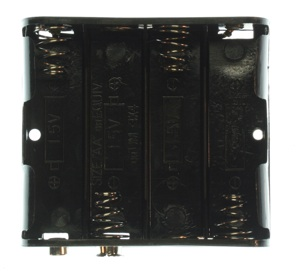
\includegraphics[scale=0.5]{img/components/battery_holder.jpg}
     \caption{AA battery holder}
     \label{AA battery holder}
\end{figure}


\begin{figure}[!htb]
     \centering
     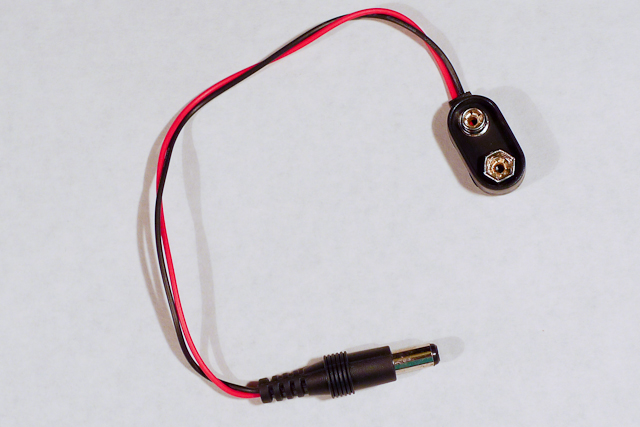
\includegraphics[scale=0.3]{img/components/battery_snap.jpg}
     \caption{9V battery snap}
     \label{9V battery snap}
\end{figure}

\section{Motors}

\subsection{Servo Motor}

\begin{figure}[!htb]
     \centering
     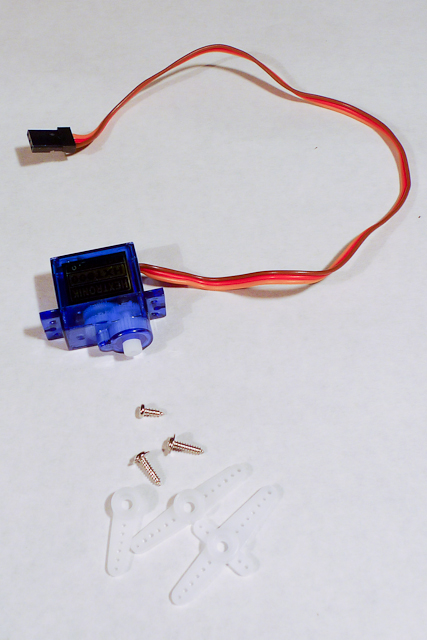
\includegraphics[scale=0.3]{img/components/servomotor.jpg}
     \caption{servomotor}
     \label{servomotor}
\end{figure}


\subsection{DC Motor}

\begin{figure}[!htb]
     \centering
     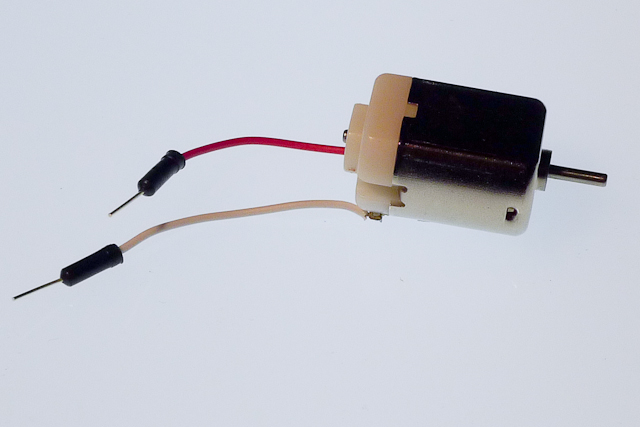
\includegraphics[scale=0.3]{img/components/dc_motor.jpg}
     \caption{DC motor}
     \label{DC motor}
\end{figure}


\section{Gear Kit}

\begin{figure}[!htb]
     \centering
     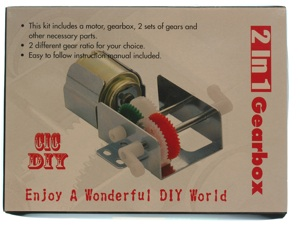
\includegraphics[scale=0.5]{img/components/gear_kit.jpg}
     \caption{gearbox kit}
     \label{LEDs}
\end{figure}


\section{H-Bridge}

\begin{figure}[!htb]
     \centering
     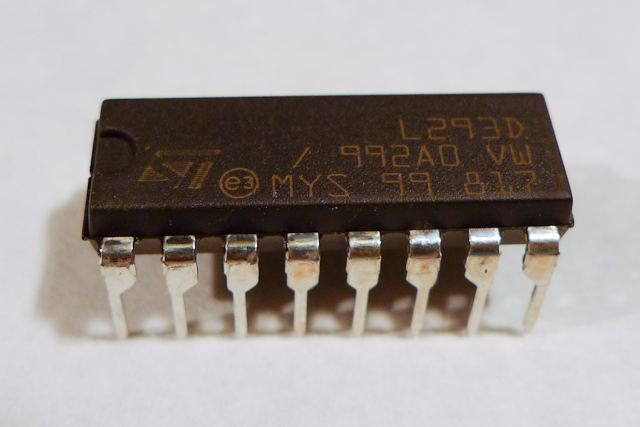
\includegraphics[scale=0.3]{img/components/h_bridge.jpg}
     \caption{H-bridge}
     \label{H-bridge}
\end{figure}


\section{Reed Relay}

\begin{figure}[!htb]
     \centering
     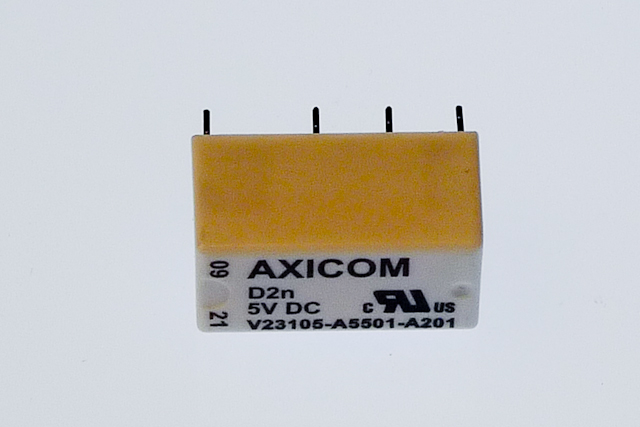
\includegraphics[scale=0.3]{img/components/relay.jpg}
     \caption{reed relay}
     \label{reed relay}
\end{figure}

\section{Screw Terminal}

\begin{figure}[!htb]
     \centering
     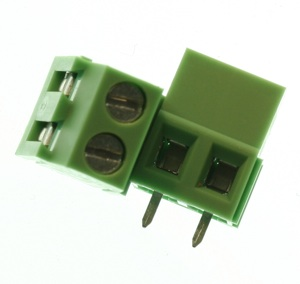
\includegraphics[scale=0.3]{img/components/screw_terminals.jpg}
     \caption{screw terminals}
     \label{screw terminals}
\end{figure}


